
\documentclass[12pt]{amsart}
\usepackage{amsmath}%
\usepackage{graphicx}
\usepackage{xcolor}
\usepackage{amssymb}
\usepackage{geometry} % see geometry.pdf on how to lay out the page. There's lots.
\geometry{a4paper} % or letter or a5paper or ... etc
% \geometry{landscape} % rotated page geometry

% See the ``Article customise'' template for come common customisations

\newcommand{\ahcomment}[1]{\textcolor{blue}{[#1 -AH]}}

\title{}
\author{}
\date{} % delete this line to display the current date

%%% BEGIN DOCUMENT
\begin{document}

\maketitle
\tableofcontents

\section{Stats}

$$
\text{Var(aX)} = a^2 Var(X)
$$

Score $\triangleq$ gradient of $\ell$ w.r.t  $\theta$.

\subsection{Markov inequality}

$$p(X\geq a) \leq \frac{E[X]}{a}$$

\begin{figure}[h]
\centering
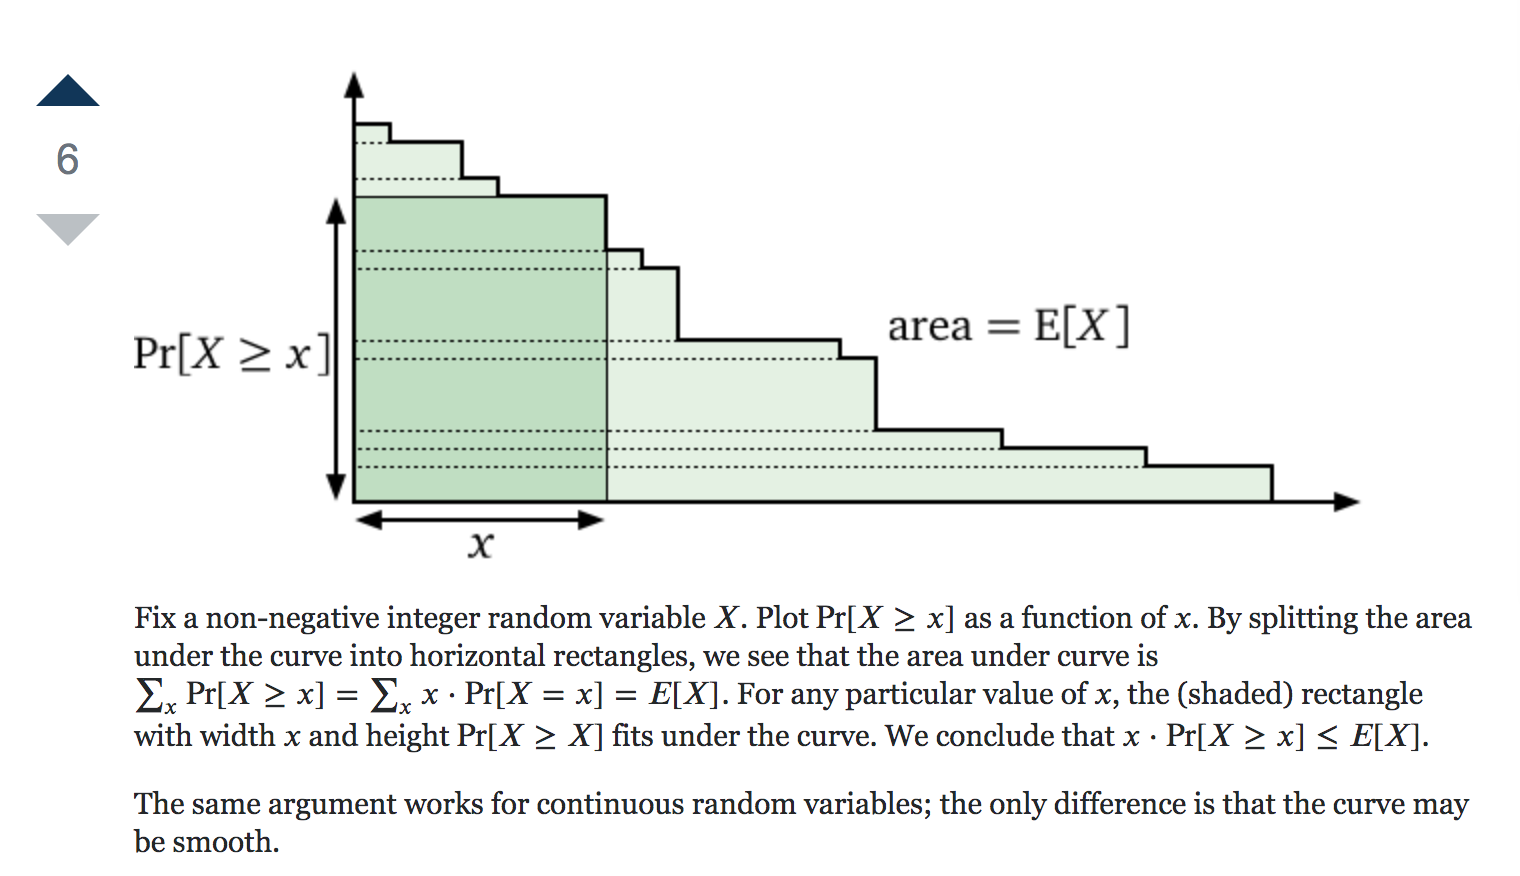
\includegraphics[width=8cm]{markov.png}
\caption{Via Stackoverflow. The $E[X]$ is easier to interpret if you convince yourself that it is a sum over the \textit{horizontal} rectangles in the picture}
\end{figure}



Mnemonic: no more than $\frac{1}{a}$ of population can have more than $a$ times the average.\footnote{https://www.quora.com/What-is-an-intuitive-explanation-of-Markovs-inequality} See also stackexchange for original graphic\footnote{https://math.stackexchange.com/questions/518873/visualizing-markov-and-chebyshev-inequalities}.

\section{Linear Algebra}

Let $A$ and $B$ be matrixes. Then $(AB)^T$ = $(B^T A^T)$. 

Pf. Let $A_i$ be the $i$th row of $A$ and $B_j$ be the $j$th column of $B$.  By definition $B_j$ is also the $j$th row of $B^T$ and $A_i$ is the $i$th column of $A^T$. Also by definition component $AB_{i,j}$ = $A_i \cdot B_j$. The definition of transpose $(AB)^T_{j,i} = AB_{i,j} = B^T_{j}A^T_i$.

Mnemonic: ``push in T, swap A and B.'' 



\section{MCMC}

Resources: mathmonk videos and murphy.

Many distributions have the form $\pi(x) = \frac{\widetilde{\pi}(x)}{Z}$ where $Z$ is expensive and $\widetilde{\pi}(x)$ is cheap.

Gibbs is a special case of MCMC where you always accept the proposal and where the proposal is the probability of some held out variable conditioned on the others.

$T$ is a transition matrix or stochastic matrix where rows sum to 1.

In Metropolis algorithm you have symmetric proposal distribution. In Metropolis-Hastings you have a Hastings correction, when the proposal is not symmetric. 

\subsection{Detailed balance}

Detailed balance intuition: $\pi_a T_{a,b} = \pi_b T_{b,a}$ $\forall a,b$

Reversibility:  Let $T$ be a transition matrix and $\pi$ be a distribution over states defining a Markov Chain (MC). Then if $(X_0, X_1 ... X_n) \sim MC(\pi, T)$ = $(X_n, X_{n -1} ... X_1) \sim MC(\pi, T)$ we say ? 

We say that a MC is reversible if there is a stationary distribution for its transition matrix. We say that a pmf satisfies DB. 

Reversibility is more specific than exchangeability. You can be reversible but not exchangeable. 

If there is some probability mass in state $a$ at time $i$ and some probability mass in state $b$ at time $i$, then $\pi_a T_{a,b} = \pi_b T_{b,a}$ for all pairs $b,a$.

Intuition: there is some mass at $a$ given by $\pi_a$. There is some mass at $b$ given by $\pi_b$. Some fraction of the mass from $a$ transitions to $b$ via $T_{a,b}$ and vice versa. 

\subsection{Metropolis algo}
Not actually derived by Metropolis. Goal is to sample from some distro $\pi$ that is complex or get the expected value of the distribution. Basically you make a MC that approximates $\pi$. 

Let $Q$ be a symmetric proposal distribution. Let $u \sim U(0,1)$ be a sample from the uniform distribution between 0, 1.

Proposal samples $x \sim Q(x_i, x)$, i.e. $p(x | x_i) \sim Q(x_i, x)$. 

If $u < \frac{\widetilde{\pi}(x)}{\widetilde{\pi}(x')}$ then $x_{i+1} = x$ else $x_{i+ 1} = x_i$.

You can show that this satisfies detailed balance. MM and Murphy have proofs. Need to return to them.

\subsection{Choosing proposals for MH}
In MH you can have any proposal you want. According to Murphy any proposal distribution is valid if it explores the whole space. More formally, the proposal must assign a non-zero probability to all places in the target distribution. I think the correction here does all of the hard work.

\subsection{Flavors of MCMC}
Independent MC is when the proposal does not depend on the state $x$: e.g. proposal is always a unit Gaussian. This shows up in IR paper from Brendan and in Dredze Eisner paper on name phylogenies. 

\section{To Learn}
Yee Whye Teh, Michael Jordan, Matthew Beal, and David Blei.
2006. Hierarchical dirichlet processes. Journal of the American Statistical Association, 101.

\end{document}